\documentclass[11pt,a4paper,fontset=none]{ctexart}
\setCJKmainfont[Path=../../assets/fonts/,AutoFakeBold=2.5,AutoFakeSlant=.2]{NotoSansSC.ttf}
\setCJKsansfont[Path=../../assets/fonts/,AutoFakeBold=2.5,AutoFakeSlant=.2]{NotoSansSC.ttf}
\setCJKmonofont[Path=../../assets/fonts/,AutoFakeBold=2.5]{NotoSansSC.ttf}
\usepackage[margin=2.3cm]{geometry}
\usepackage{amsmath,amssymb}
\usepackage{booktabs,longtable,array}
\usepackage{graphicx}
\usepackage{xcolor}
\usepackage{listings}
\usepackage{fancyhdr}
\usepackage{hyperref}
\usepackage{enumitem}
\usepackage{caption}
\usepackage{subcaption}
\usepackage{float}
\usepackage{seqsplit}
\hypersetup{colorlinks=true,linkcolor=blue!55!black,urlcolor=blue!65!black,citecolor=blue!55!black}
\urlstyle{same}
\setlength{\parindent}{2em}
\setlength{\parskip}{0.25em}
\setlength{\headheight}{14pt}
\setlength{\emergencystretch}{2em}
\pagestyle{fancy}
\fancyhf{}
\lhead{Bitcoin 实验一：Testnet4 交易与区块解析}
\rhead{\thepage}
\definecolor{labblue}{HTML}{2457A6}
\definecolor{labgreen}{HTML}{16825D}
\definecolor{laborange}{HTML}{C66A14}
\definecolor{codebg}{HTML}{F5F7FA}
\lstset{basicstyle=\ttfamily\small,backgroundcolor=\color{codebg},frame=single,breaklines=true,columns=fullflexible,showstringspaces=false}

\title{\bfseries Bitcoin Testnet4 交易构造与完整区块逐字节解析\\[0.5em]
\large 课程实验报告（真实链上交易与完整区块验证版）}
\author{Bitcoin 实验一}
\date{2026 年 7 月 20 日}

\begin{document}
\maketitle

\begin{abstract}
本实验实现了一个不依赖本地全节点的 Bitcoin Testnet4 实验工具：本地生成一次性 secp256k1 密钥，手工构造并签名原生 SegWit P2WPKH 交易，通过 Esplora API 查询 UTXO、广播和下载完整区块，并将交易与区块的每一个字节映射到字段、端序、8-bit 表示和语义。真实实验交易 \texttt{fda3dd67\ldots c3666428} 已确认在高度 144927；本地重算的 BIP143 摘要、ECDSA 签名、TXID、WTXID 与金额守恒全部通过。包含该交易的区块共 88,989 bytes、29 笔交易，解析器生成 88,989 条无缺口覆盖记录，并独立验证 block hash、Merkle root 与 Proof of Work。报告同时保留 faucet 失败、成功领取、待确认和最终确认截图，使过程与最终结果均可复查。

\textbf{关键词：} Bitcoin；Testnet4；P2WPKH；BIP143；SegWit；区块序列化；Bitcoin Script
\end{abstract}

\clearpage
\tableofcontents
\newpage

\section{实验目标与完成状态}

实验目标包括真实测试网交易、交易逐字段解析、完整区块解析、locking/unlocking data 分析以及 PoW 计算。当前结果如表 \ref{tab:status}。

\begin{table}[htbp]
\centering
\caption{实验完成状态}
\label{tab:status}
\begin{tabular}{p{0.27\textwidth}p{0.18\textwidth}p{0.45\textwidth}}
\toprule
项目 & 状态 & 证据 \\
\midrule
Python 手写解析器 & 完成 & 17 个单元测试全部通过 \\
双地址一次性钱包 & 完成 & 私钥文件权限为 0600，公开地址单独保存 \\
真实完整区块解析 & 完成 & 最终区块高度 144927，88,989 字节，29 笔交易 \\
Merkle root 与 PoW & 完成 & 本地计算均为 true \\
自建交易签名逻辑 & 完成 & BIP143、DER、low-S、TXID/WTXID 均有测试 \\
自建交易广播与确认 & 完成 & 高度 144927，交易、Merkle、PoW 全部验证通过 \\
\bottomrule
\end{tabular}
\end{table}

\section{实验环境与安全设计}

\begin{table}[H]
\centering
\caption{任务一本机实验环境}
\label{tab:task1-environment}
\begin{tabular}{p{0.24\textwidth}p{0.66\textwidth}}
\toprule
项目 & 配置 \\
\midrule
硬件 & MacBook Pro（Mac14,9），Apple M2 Pro 10-core，16 GB memory \\
操作系统 & macOS 15.6.1，ARM64 \\
Python & CPython 3.13.3 \\
密码学实现 & \texttt{coincurve 21.0.0}，底层使用 \texttt{libsecp256k1} \\
区块链网络 & Bitcoin Testnet4，native SegWit P2WPKH \\
公共数据接口 & mempool.space Testnet4 Esplora API：\url{https://mempool.space/testnet4/api} \\
测试工具 & pytest 8.4.2，共 17 个单元测试 \\
报告工具 & XeLaTeX、\texttt{ctexart}、\texttt{latexmk}、Poppler \\
\bottomrule
\end{tabular}
\end{table}

发送地址与接收地址均为本实验新建的一次性 native SegWit 地址：

\begin{description}[style=nextline]
  \item[Sender] \url{tb1qjgfszrz7926jglm0nc702605zh0w2qe9ryr06d}
  \item[Receiver] \url{tb1qu75gwqg4gdfdfurvfxv77trwq9dt6zzgnh2ys5}
\end{description}

私钥仅写入被忽略的 \texttt{.secrets/testnet4\_wallet.json}，报告、截图、CSV 与 JSON 均不含私钥。脚本重复执行 \texttt{wallet-init} 时只读取既有钱包，不覆盖密钥。

\section{序列化规范与实现不变量}

Bitcoin 的线格式并不是把一个 JSON 对象直接编码，而是由定长整数、CompactSize、定长哈希和变长字节串依次拼接。解析器必须同时处理“线上的字节顺序”和 explorer 面向人的展示顺序；如果二者混用，即使字段看起来正确，TXID、block hash 与 Merkle root 也会全部错误。表 \ref{tab:serialization-rules} 汇总了本实验实际使用的编码规则。

\begin{table}[H]
\centering
\caption{交易与区块解析使用的基础序列化规则}
\label{tab:serialization-rules}
\begin{tabular}{p{0.22\textwidth}p{0.31\textwidth}p{0.37\textwidth}}
\toprule
数据类型 & 线格式 & 本实验的处理 \\
\midrule
定长整数 & version、vout、amount、sequence、locktime 等使用 little-endian & 先保留原始十六进制，再按字段宽度解码为整数 \\
32-byte hash & outpoint 中以前一交易哈希的内部字节序保存 & 显示 TXID/block hash 时翻转 32 bytes；参与哈希时使用规范序列化字节 \\
CompactSize & $0\ldots252$ 直接编码；之后用 \texttt{fd}/\texttt{fe}/\texttt{ff} 加 2/4/8-byte little-endian & 检查截断与 non-canonical encoding，并覆盖 252/253、65,535/65,536 边界 \\
变长字节串 & CompactSize 长度后紧跟指定数量字节 & scriptSig、scriptPubKey 和 witness item 均先读取长度，再进行边界检查 \\
SegWit 标志 & version 后出现 \texttt{00 01} & marker/flag 属于完整序列化，但不属于 stripped serialization \\
\bottomrule
\end{tabular}
\end{table}

对同一笔 SegWit 交易，完整序列化记为 $S_{\mathrm{full}}$，删除 marker、flag 与 witness 后的传统序列化记为 $S_{\mathrm{base}}$。本实验按 Bitcoin 的展示约定计算
\begin{align*}
 \mathrm{TXID}  &= \operatorname{reverse}\!\left(\operatorname{SHA256d}(S_{\mathrm{base}})\right),\\
 \mathrm{WTXID} &= \operatorname{reverse}\!\left(\operatorname{SHA256d}(S_{\mathrm{full}})\right).
\end{align*}
本次交易的 base size 为 113 bytes，witness serialization（含 marker/flag）为 110 bytes，因此
\[
 \mathrm{weight}=4\times113+110=562\ \mathrm{WU},\qquad
 \mathrm{vsize}=\left\lceil\frac{562}{4}\right\rceil=141\ \mathrm{vB}.
\]
这也解释了为什么同一笔交易的 TXID 与 WTXID 不同，以及为什么手续费率按 vB 而非原始 223 bytes 计价。

解析器把游标单调前移作为核心不变量：每次读取都必须先证明剩余长度足够；每个半开区间 $[\textit{offset\_start},\textit{offset\_end})$ 只能被一个字段消费；解析结束时游标必须恰好等于输入长度。逐字节 CSV 是这些不变量的外部证明，而不是解析完成后的附加格式化结果。

\section{交易构造与签名方法}

\subsection{P2WPKH 输出与地址}

压缩公钥 $P$ 先计算
\[
 h=\operatorname{RIPEMD160}(\operatorname{SHA256}(P)),
\]
输出脚本为 \texttt{00 14 <20-byte h>}，地址使用 Testnet4 的 \texttt{tb} HRP 进行 Bech32 编码。实验交易固定为 version 2、一个输入、付款与找零两个 P2WPKH 输出、\texttt{sequence=0xfffffffd}（opt-in RBF）和 \texttt{locktime=0}。

\subsection{BIP143 摘要}

对输入 $i$，实现的 SegWit v0 签名预映像为
\begin{align*}
&nVersion \parallel hashPrevouts \parallel hashSequence \parallel outpoint_i\\
&\parallel scriptCode_i \parallel value_i \parallel sequence_i\\
&\parallel hashOutputs \parallel nLockTime \parallel sighashType.
\end{align*}
最终摘要是该预映像的 double-SHA256。P2WPKH 的 \texttt{scriptCode} 还原为传统 P2PKH 形式
\[
\texttt{76 a9 14 <HASH160(pubkey)> 88 ac}.
\]
其中三个聚合哈希分别为
\begin{align*}
 hashPrevouts &= \operatorname{SHA256d}(outpoint_0\parallel\cdots\parallel outpoint_{n-1}),\\
 hashSequence &= \operatorname{SHA256d}(sequence_0\parallel\cdots\parallel sequence_{n-1}),\\
 hashOutputs  &= \operatorname{SHA256d}(output_0\parallel\cdots\parallel output_{m-1}).
\end{align*}
\texttt{SIGHASH\_ALL} 把全部输入 outpoint、全部 sequence 和全部输出承诺进摘要；当前输入的 outpoint、\texttt{scriptCode} 与 UTXO 金额则显式出现在预映像中。SegWit v0 把被花费金额纳入摘要，使离线签名器无需获取整笔前序交易也能检测被替换的输入金额。对本实验数据重建出的摘要为
\[
\texttt{\seqsplit{e2c574443348d600e3e03aaabd23ea731fdde9a580f3a07a32aeb96e1f9c338c}}.
\]

签名采用 ECDSA、DER 编码、low-S 规范化并在末尾附加 \texttt{01}（\texttt{SIGHASH\_ALL}）。native P2WPKH 输入的 \texttt{scriptSig} 为空；真正的 unlocking data 是 witness 中的签名与压缩公钥，而 witness item 本身不是一段需要逐 opcode 执行的 Script。

\subsection{ECDSA、DER 与 low-S 的实证检查}

令 secp256k1 基点为 $G$、阶为 $n$、公钥为 $P=dG$，摘要解释为标量 $e$。验证端计算
\[
w=s^{-1}\bmod n,\qquad u_1=ew\bmod n,\qquad u_2=rw\bmod n,
\]
再检查点 $R'=u_1G+u_2P$ 的横坐标是否满足 $x(R')\bmod n=r$。本实验没有把库返回的“验证成功”当作唯一证据：程序从 witness 取出 DER、分离最后一个 sighash byte、重新计算 $e$，再使用 witness 中的压缩公钥执行上述验证。

本次 witness 公钥为
\begin{lstlisting}[language={}]
021c2a98e839fb46a75c19528a8e7466c41ffa4639ac3db717963c8355d3a7dec8
\end{lstlisting}
签名中两个 DER 整数为
\begin{align*}
r&=\texttt{af0175f0222620ee9264406ccaccdbe1277442e3247808dcd697dcdfb29d9478},\\
s&=\texttt{25a183f8a647ac59ee66a4409a6756c80f1467a50be2f11048fef9f71a1f4f8b}.
\end{align*}
DER 外的末字节 \texttt{01} 表示 \texttt{SIGHASH\_ALL}。$s$ 已满足 $1\le s\le n/2$；low-S 把数学上同样有效的 $(r,n-s)$ 排除，减少仅改变签名编码而不改变支付语义的可塑性。DER 中 $r$ 的最高位为 1，因而编码前有一个 \texttt{00} 正号字节；解析器按 ASN.1 INTEGER 规则验证该字节是否必要，并拒绝多余前导零、负数和长度不一致。

\subsection{金额与费用}

默认付款 1,000 sats，费率 2 sat/vB。脚本选择一个已确认 UTXO，并计算
\[
\text{change}=\text{input}-\text{payment}-\lceil 2\times vsize\rceil.
\]
若付款或找零低于保守 dust threshold 294 sats，程序在签名前拒绝构造。广播前再次验证签名、摘要、金额守恒、TXID 和 WTXID。

\section{真实实验交易结果}

CypherFaucet 向 sender 注入 1,000,000 sats；入账交易 TXID 为
\texttt{\seqsplit{a7619af457e75fc4c4f51fc1d0d4fe849885274d33ffccb0b47fb75f3a8cace2}}，
其 vout 0 在高度 144925 确认。随后本地程序使用该 UTXO 构造、签名并广播实验交易。交易核心结果如下：

\begingroup
\setlength{\tabcolsep}{3pt}
\begin{longtable}{p{0.27\textwidth}p{0.68\textwidth}}
\toprule
字段 & 结果 \\
\midrule
TXID & \scriptsize\texttt{\seqsplit{fda3dd67e4516d68c4f023a43c7a92629b9262d7e816d09cae873907c3666428}} \\
WTXID & \scriptsize\texttt{\seqsplit{dbebb2a01ab826570124b004a33d6da4a14f552dfbb29323a7520d7a9f1d1fba}} \\
输入 & 1,000,000 sats，faucet UTXO vout 0 \\
付款输出 & 1,000 sats，发送至 receiver P2WPKH \\
找零输出 & 998,718 sats，返回 sender P2WPKH \\
手续费 / 费率 & 282 sats / 2.00 sat/vB（explorer 显示 2.01 sat/vB）\\
Size / base / weight / vsize & 223 B / 113 B / 562 WU / 141 vB \\
Version / sequence / locktime & 2 / \texttt{0xfffffffd} / 0 \\
scriptSig & 空（native P2WPKH）\\
Witness & 两项：DER+\texttt{SIGHASH\_ALL} 签名、33-byte 压缩公钥 \\
BIP143 digest & \scriptsize\texttt{\seqsplit{e2c574443348d600e3e03aaabd23ea731fdde9a580f3a07a32aeb96e1f9c338c}} \\
本地验证 & signature、sighash、TXID、WTXID、金额守恒全部为 true \\
Byte coverage & 223 records，complete=true \\
\bottomrule
\end{longtable}
\endgroup

交易输出金额满足
\[
1{,}000{,}000 = 1{,}000 + 998{,}718 + 282.
\]
其中 marker/flag 为 \texttt{00 01}；输入的 \texttt{scriptSig} 长度为零，witness 单独序列化，因此 TXID 排除 witness，而 WTXID 包含 witness。CSV 中 223 条记录与 223 个原始字节一一对应。

从字节布局看，offset 0--3 是 version，4--5 是 marker/flag，offset 6 的 \texttt{01} 是输入数；唯一输入随后给出反序保存的前序 TXID、vout 0、长度为零的 scriptSig 与 \texttt{fdffffff} sequence。两个输出分别携带 1,000 和 998,718 sats，且 scriptPubKey 都是 22-byte 的 \texttt{00 14 <20-byte key hash>}。输出之后才出现 witness stack：计数 \texttt{02}、72-byte 签名项与 33-byte 压缩公钥项，最后四字节为 locktime。该顺序既能从 raw hex 单独恢复，也与生成的逐字节 JSON/CSV 一致。

\section{逐字节解析器}

\subsection{交易字段}

解析顺序严格跟随 consensus serialization：version，SegWit marker/flag，CompactSize input count，inputs，output count，outputs，witnesses 和 locktime。每个被消费的字节产生一条记录：

\begin{lstlisting}[language={},caption={逐字节 CSV 数据契约}]
offset_start, offset_end, raw_hex, bits,
field_path, decoded_value, endian, notes
\end{lstlisting}

覆盖断言要求 offset 恰好为 $0,1,\ldots,N-1$，不得有缺口或重复。CompactSize 特别测试 252/253、65,535/65,536 边界，并拒绝 non-canonical encoding。

\subsection{Script 处理范围}

工具能识别 P2PKH、P2SH、P2WPKH、P2WSH、P2TR、OP\_RETURN，解析直接 push、OP\_PUSHDATA1/2/4，并保留未知 opcode。对本实验 P2WPKH 输入执行完整的摘要重建与 ECDSA 验证；对完整区块中的其他脚本做结构化反汇编，但不声称替代 Bitcoin Core 的完整共识 Script VM。

\begin{table}[H]
\centering
\setlength{\tabcolsep}{3pt}
\caption{解析器覆盖的常见输出脚本与解锁数据位置}
\label{tab:script-patterns}
\begin{tabular}{p{0.13\textwidth}p{0.40\textwidth}p{0.37\textwidth}}
\toprule
类型 & 典型 locking script / witness program & spending input 的主要数据 \\
\midrule
P2PKH & \texttt{OP\_DUP OP\_HASH160 <20B> OP\_EQUALVERIFY OP\_CHECKSIG} & scriptSig 中的签名与公钥 \\
P2SH & \texttt{OP\_HASH160 <20B> OP\_EQUAL} & scriptSig 最后一项为 redeemScript；具体参数位于其前 \\
P2WPKH & \texttt{OP\_0 <20B keyhash>} & scriptSig 为空；witness 为签名、公钥 \\
P2WSH & \texttt{OP\_0 <32B scripthash>} & witness 最后一项为 witnessScript \\
P2TR & \texttt{OP\_1 <32B x-only key>} & witness 为 key-path 签名，或 script-path 参数、脚本与 control block \\
OP\_\allowbreak RETURN & \texttt{OP\_RETURN <data>} & 可证明不可花费，用于承载有限元数据 \\
\bottomrule
\end{tabular}
\end{table}

“反汇编”与“验证”在本报告中严格区分：前者把 opcode 和 data-push 边界恢复为结构化记录，未知 opcode 也不丢失；后者需要执行签名摘要规则与 Script 语义。本实验只对自身 P2WPKH 输入实现完整验证闭环，对区块内其他脚本不推断其历史执行上下文。

\section{先验公开区块解析结果}

本实验下载并解析区块高度 144877：

\begingroup
\setlength{\tabcolsep}{3pt}
\begin{longtable}{p{0.27\textwidth}p{0.68\textwidth}}
\toprule
字段 & 结果 \\
\midrule
Block hash & \scriptsize\texttt{\seqsplit{0000000000e9ed9d48999d673d817cf089298e111083a71670cc7c6b4faf856d}} \\
Previous block & \scriptsize\texttt{\seqsplit{0000000000865d144d99fc51ed2ab39490e3eb144038c0ea7b5cd71ed7369dcf}} \\
Merkle root & \scriptsize\texttt{\seqsplit{0588d2c1047631a0859060c5ecfe9c6e46440f28f60bb7bbf3aaf12417b348f7}} \\
Size / transactions & 4,537 bytes / 19 transactions \\
Bits / nonce & \texttt{1d00ffff} / 4,083,417,704 \\
Coinbase height & 144877（由 coinbase scriptSig 首个 push 解码）\\
Witness commitment & \scriptsize\texttt{\seqsplit{6c4a8c9288478cb4dcd419245d0ef4f8901c75cbd55e7761fe3f51c05668c69b}} \\
Byte coverage & 4,537 records，complete=true \\
Merkle / PoW & true / true \\
\bottomrule
\end{longtable}
\endgroup

80-byte header 原始十六进制为：
\begin{lstlisting}[language={}]
00801022 cf9d36d71ed75c7beac0384014ebe39094b32aed51fc994d145d860
00000000 f748b31724f1aaf3bbb70bf6280f44466e9cfeecc5609085a031760
4c1d2880 5a4eb5d6 ffff001d 680264f3
\end{lstlisting}

本地计算 $H=\operatorname{SHA256d}(header)$，按展示约定翻转后得到上述 block hash。\newline
由 \texttt{bits=0x1d00ffff} 得目标
\[
T=\texttt{00000000ffff0000}\ldots\texttt{0000},
\]
且 $\operatorname{int}(H)\le T$。19 个 TXID 按区块顺序逐层 double-SHA256（奇数层复制末节点）得到与 header 相同的 Merkle root。

该较小区块用于在 faucet 到账前完成集成测试。最终验收则使用下面包含本实验交易的区块，解析流程完全相同。

\section{包含实验交易的最终确认区块}

实验交易确认于高度 144927，在区块交易数组中的 0-based index 为 7（即含 coinbase 在内的第 8 笔）。关键结果如下：

\begingroup
\setlength{\tabcolsep}{3pt}
\begin{longtable}{p{0.27\textwidth}p{0.68\textwidth}}
\toprule
字段 & 结果 \\
\midrule
Block hash & \scriptsize\texttt{\seqsplit{0000000000000000bb15b540dec2b41e6d2ce74775a6c90c6eaf307377309255}} \\
Previous block & \scriptsize\texttt{\seqsplit{0000000000c7cc42a40e338d6b1f6eb3b6a8ff3d35c910094d403c3d6b0f903c}} \\
Merkle root & \scriptsize\texttt{\seqsplit{05a44f2cfa6f3903f74f1e9869019430b804dcc21167ea3b7209773e7dcf51ad}} \\
Size / transactions & 88,989 bytes / 29 transactions \\
Bits / nonce & \texttt{190228f4} / 1,680,841,051 \\
Target & \scriptsize\texttt{\seqsplit{000000000000000228f400000000000000000000000000000000000000000000}} \\
Coinbase height & 144927（由 coinbase scriptSig 首个 push 解码）\\
Witness commitment & \scriptsize\texttt{\seqsplit{18da3384b53405183de0b2aa1e19ebc349d6718a98cee96c365adc88e9502bfa}} \\
实验交易位置 & index 7，transaction\_in\_block=true \\
Byte coverage & 88,989 records，complete=true \\
Merkle / PoW & true / true \\
\bottomrule
\end{longtable}
\endgroup

80-byte header 原始十六进制为：
\begin{lstlisting}[language={}]
00401f25 3c900f6b3d3c404d0910c9353dffa8b6b36e1f6b8d330ea4
42ccc70000000000 ad51cf7d3e7709723bea6711c2dc04b83094016998
1e4ff703396ffa2c4fa405 84515e6a f4280219 5b992f64
\end{lstlisting}

本地对 header 做 double-SHA256 并按展示端序反转后得到 block hash；由 compact target \texttt{0x190228f4} 展开得到表中 $T$，验证 $\operatorname{int}(H)\le T$。29 个 TXID 逐层构造的 Merkle root 与 header 完全相同。block header 时间戳比实验机器当时的墙钟时间约快两小时，因此 explorer 截图出现“2 小时之后”的文案；这来自区块头时间而非确认失败，API 的 confirmed、height 与 block hash 均一致。

\subsection{区块头、Merkle 树与 witness commitment 的独立证明}

compact target 的最高字节是指数 $E=\texttt{0x19}=25$，后 3 bytes 是系数 $C=\texttt{0x0228f4}$，故
\[
T=C\times 256^{E-3}
=\texttt{000000000000000228f4}\underbrace{\texttt{00\ldots00}}_{22\ \text{bytes}}.
\]
程序把 header 的 double-SHA256 解释为 256-bit 无符号整数并验证其不大于 $T$。这一步验证的是该具体 header 是否满足声明的工作量目标；它不依赖 explorer 返回的“valid”字段。

Merkle 树从区块内 29 个 TXID 的内部哈希字节开始。每层把相邻两个节点拼接后计算 $\operatorname{SHA256d}$；若某层节点数为奇数，则复制最后一个节点。重复到单一根节点后，与 header 中的 32 bytes 逐字节比较。实验交易位于 index 7，其完整序列化在区块 raw data 的 offset 28,154--28,377，说明“交易属于该区块”不仅由 API 元数据声称，也由区块字节本身恢复。

coinbase scriptSig 的第一个 data-push 为 \texttt{03 1f 36 02}：\texttt{03} 是长度，little-endian 整数 \texttt{1f3602} 解码为 BIP34 高度 144927。coinbase 还包含形如 \texttt{6a24aa21a9ed<32B>} 的承诺输出。验证 witness commitment 时，程序把 coinbase 的 wtxid 视为 32-byte 零值，使用全区块 wtxid 构造 witness Merkle root，再计算
\[
\operatorname{SHA256d}(witness\_merkle\_root\parallel witness\_reserved\_value).
\]
该区块 coinbase witness 的 reserved value 为 32-byte 零值，计算结果为
\texttt{\seqsplit{18da3384b53405183de0b2aa1e19ebc349d6718a98cee96c365adc88e9502bfa}}，与 OP\_RETURN 承诺逐字节一致。

\begin{figure}[H]
\centering
\begin{subfigure}[t]{0.48\textwidth}
  \centering
  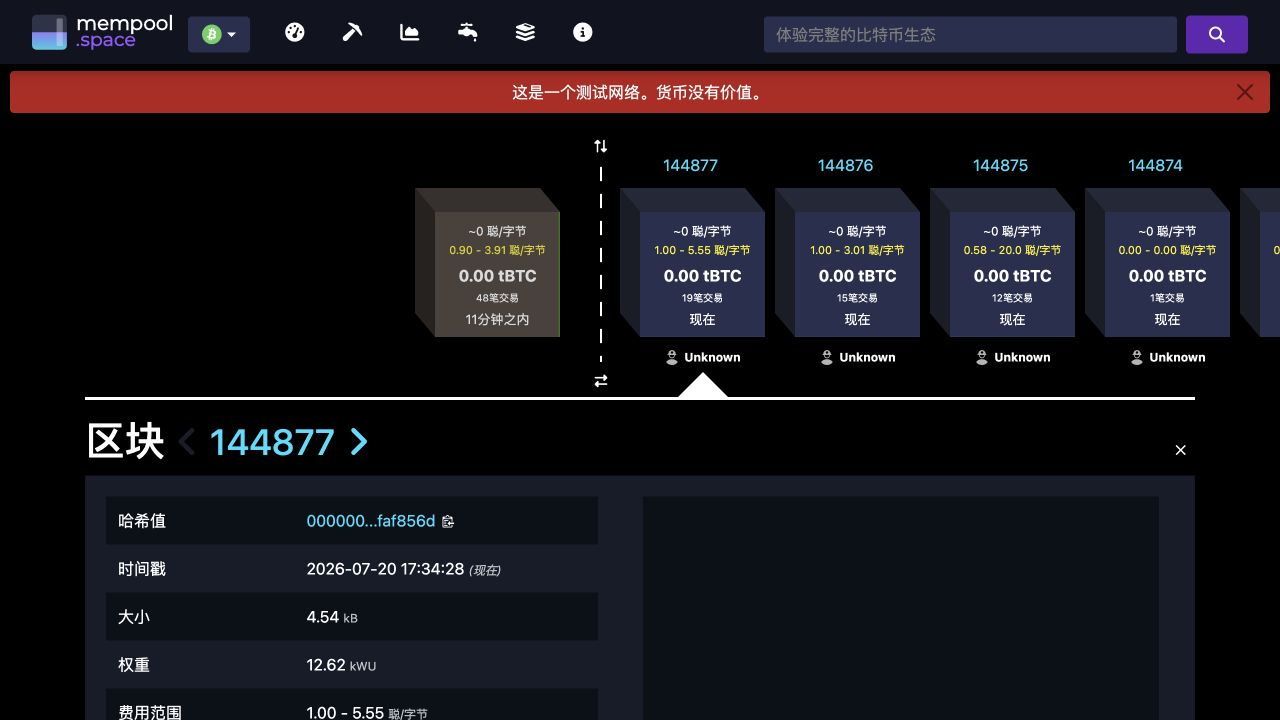
\includegraphics[width=\linewidth,height=0.20\textheight,keepaspectratio]{assets/testnet4_block_144877.png}
  \caption{先验集成测试区块：高度 144877}
\end{subfigure}\hfill
\begin{subfigure}[t]{0.48\textwidth}
  \centering
  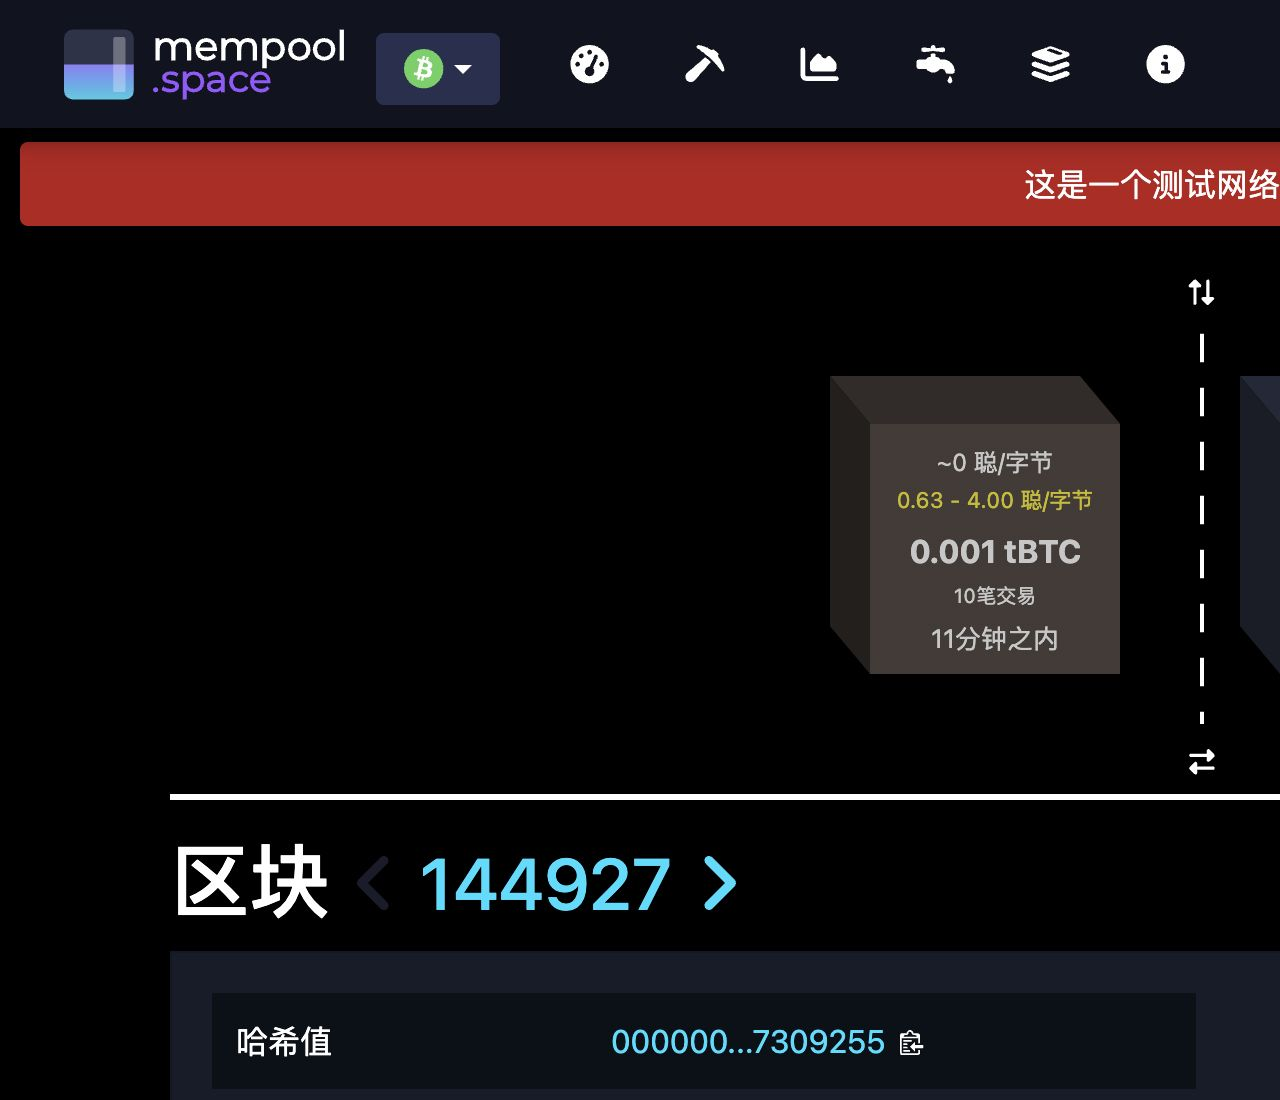
\includegraphics[width=\linewidth,height=0.20\textheight,keepaspectratio]{assets/testnet4_experiment_block_header.png}
  \caption{包含实验交易的最终区块：高度 144927}
\end{subfigure}
\caption{mempool.space 上的先验区块与最终确认区块对照；完整哈希由 API 数据和本地解析结果给出}
\label{fig:block-comparison}
\end{figure}

\section{Faucet 与广播过程记录}

mempool.space faucet 在登录后提示账户无权限；testnet4.dev faucet 的 hCaptcha 已通过，但页面同时显示无法读取 faucet balance，提交返回错误。随后改用 CypherFaucet，在不暴露私钥的前提下向公开 sender 地址申请资金，最终收到并确认 1,000,000 sats。失败与成功两类截图均保留，以证明实验过程没有用模拟 TXID 替代真实链上结果。

\begin{figure}[H]
\centering
\begin{subfigure}[t]{0.48\textwidth}
  \centering
  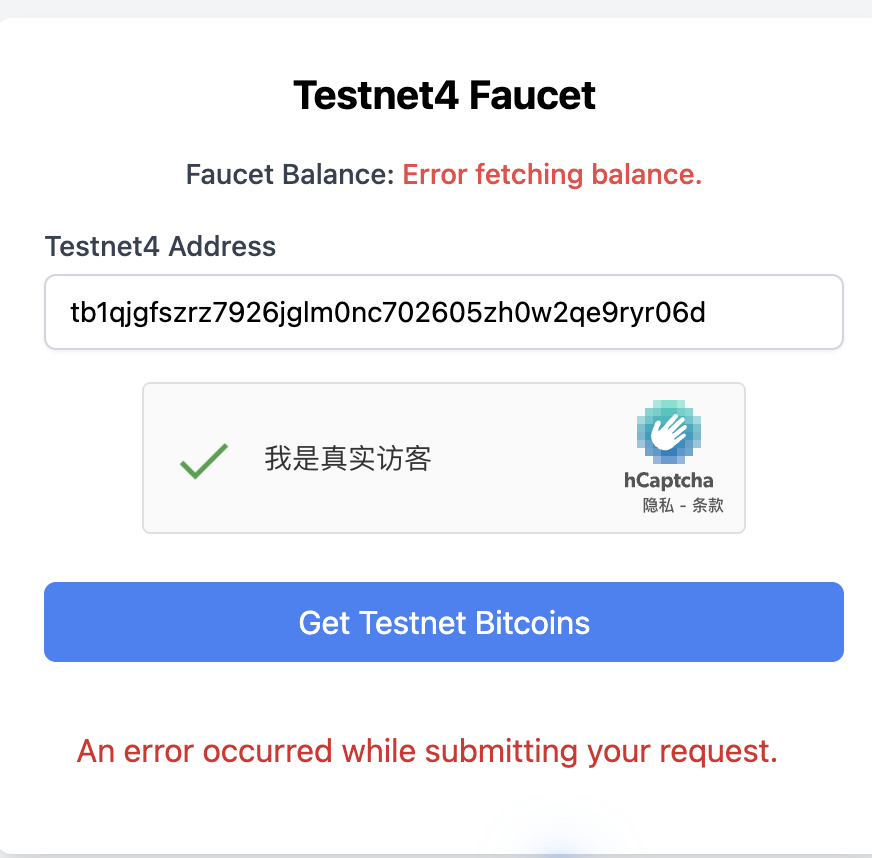
\includegraphics[width=\linewidth,height=0.27\textheight,keepaspectratio]{assets/testnet4_faucet_error.png}
  \caption{testnet4.dev：验证码通过，但后端提交失败}
  \label{fig:faucet-error}
\end{subfigure}\hfill
\begin{subfigure}[t]{0.48\textwidth}
  \centering
  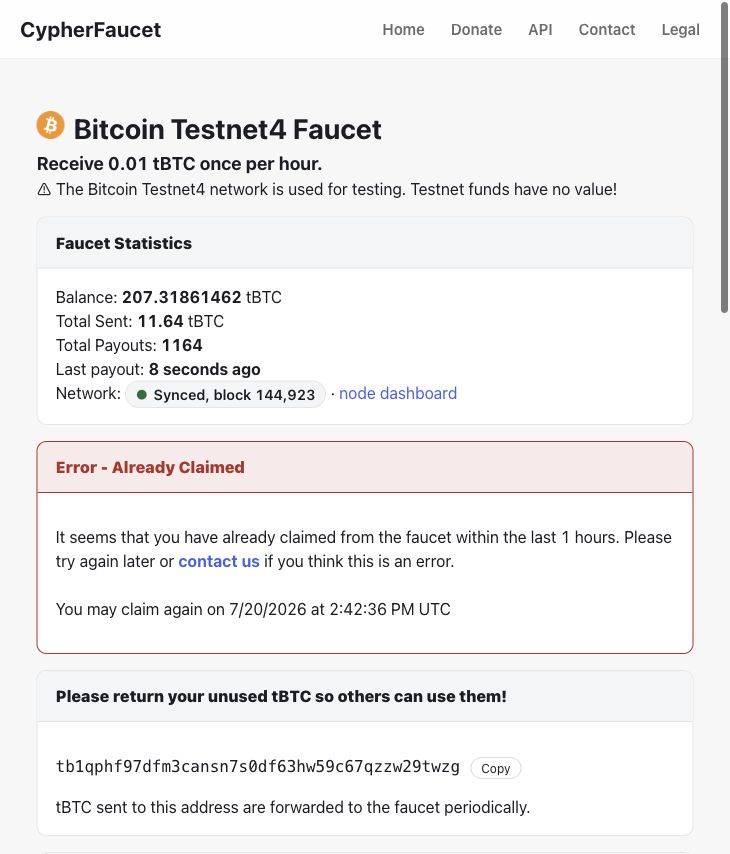
\includegraphics[width=\linewidth,height=0.27\textheight,keepaspectratio]{assets/testnet4_cypherfaucet_claimed.png}
  \caption{CypherFaucet：公开地址领取完成}
\end{subfigure}
\caption{Faucet 尝试过程：失败记录与成功领取记录并列保留}
\end{figure}

\begin{figure}[H]
\centering
\begin{subfigure}[t]{0.48\textwidth}
  \centering
  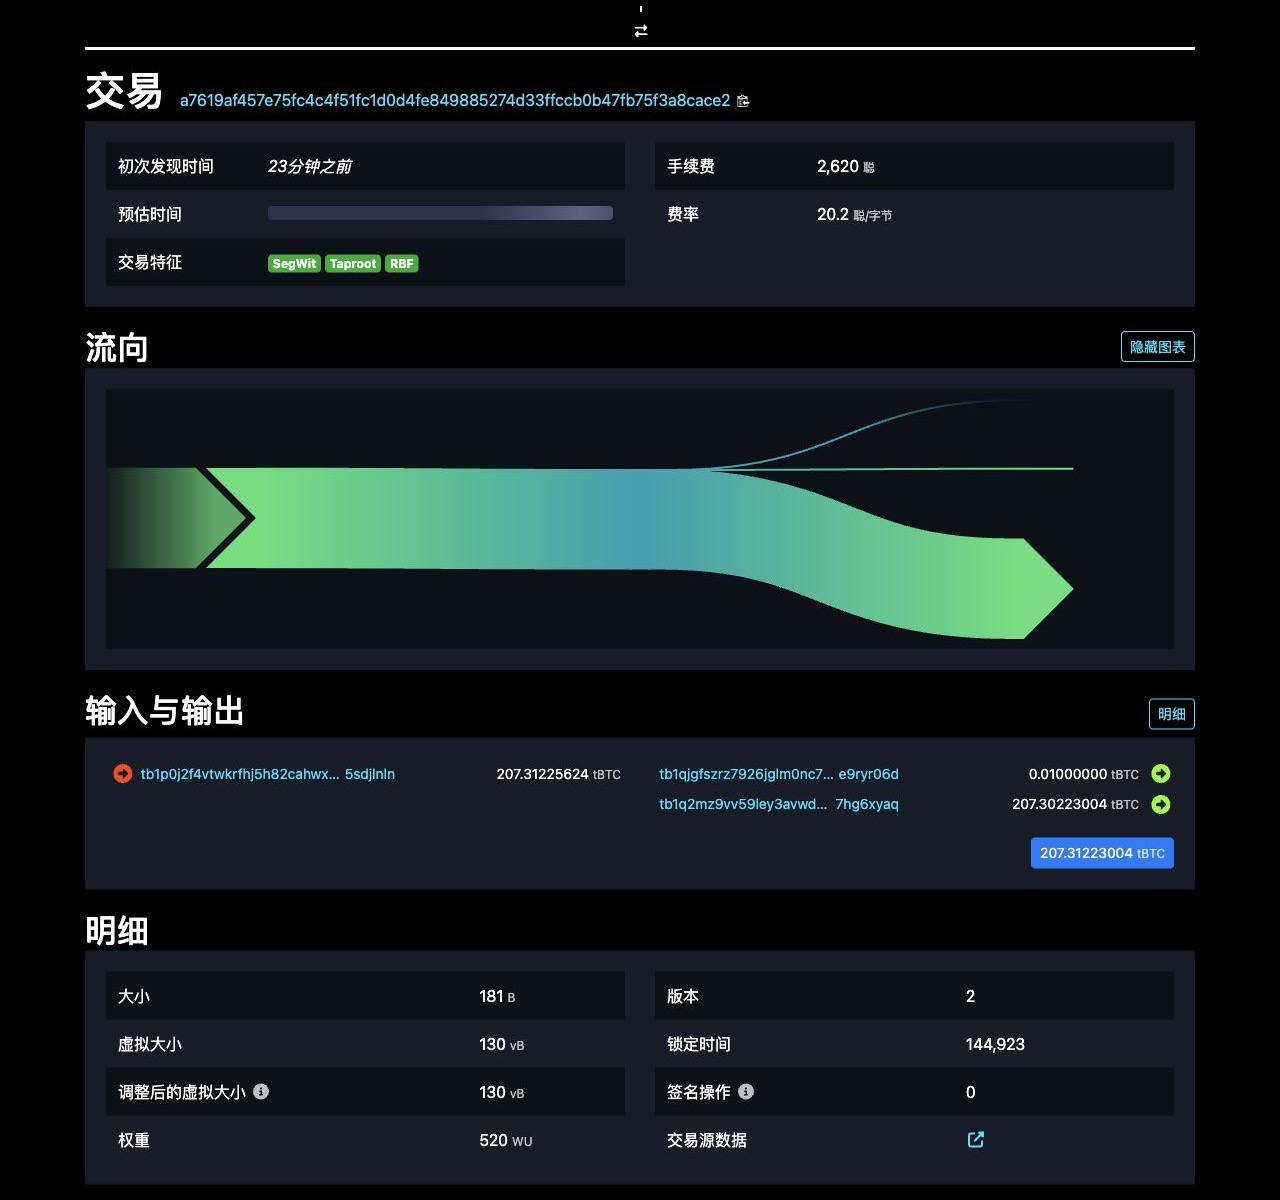
\includegraphics[width=\linewidth,height=0.20\textheight,keepaspectratio]{assets/testnet4_funding_tx_unconfirmed.png}
  \caption{Faucet 入账交易进入公开 mempool}
\end{subfigure}\hfill
\begin{subfigure}[t]{0.48\textwidth}
  \centering
  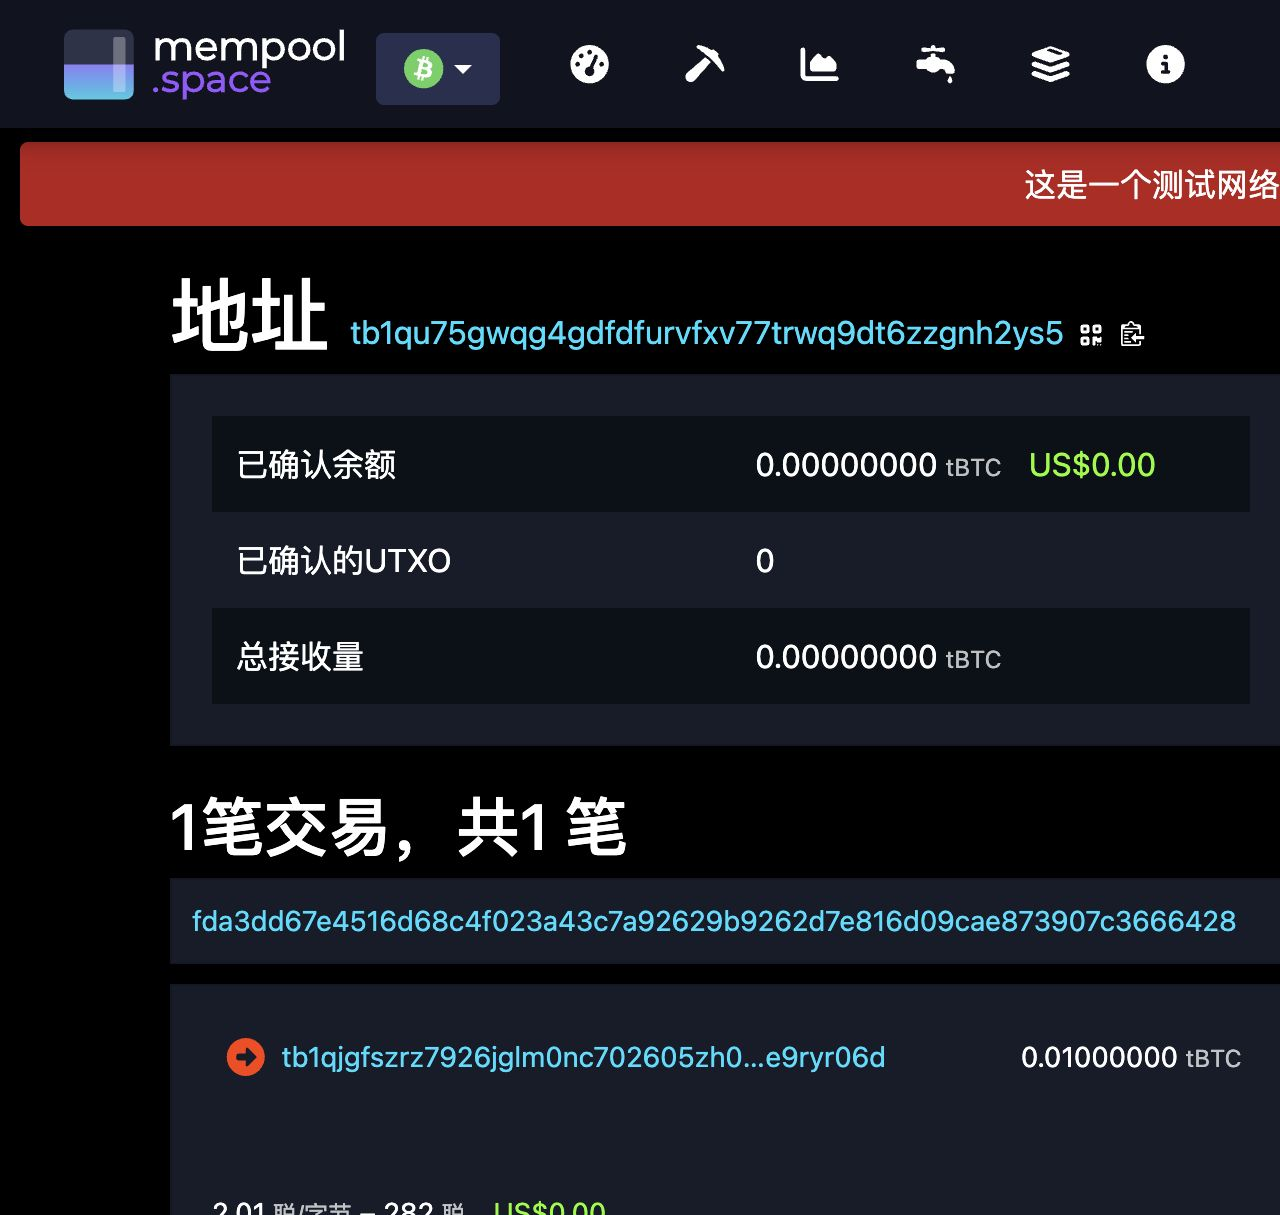
\includegraphics[width=\linewidth,height=0.20\textheight,keepaspectratio]{assets/testnet4_receiver_pending.png}
  \caption{Receiver 出现待确认的 1,000 sats}
\end{subfigure}

\medskip

\begin{subfigure}[t]{0.48\textwidth}
  \centering
  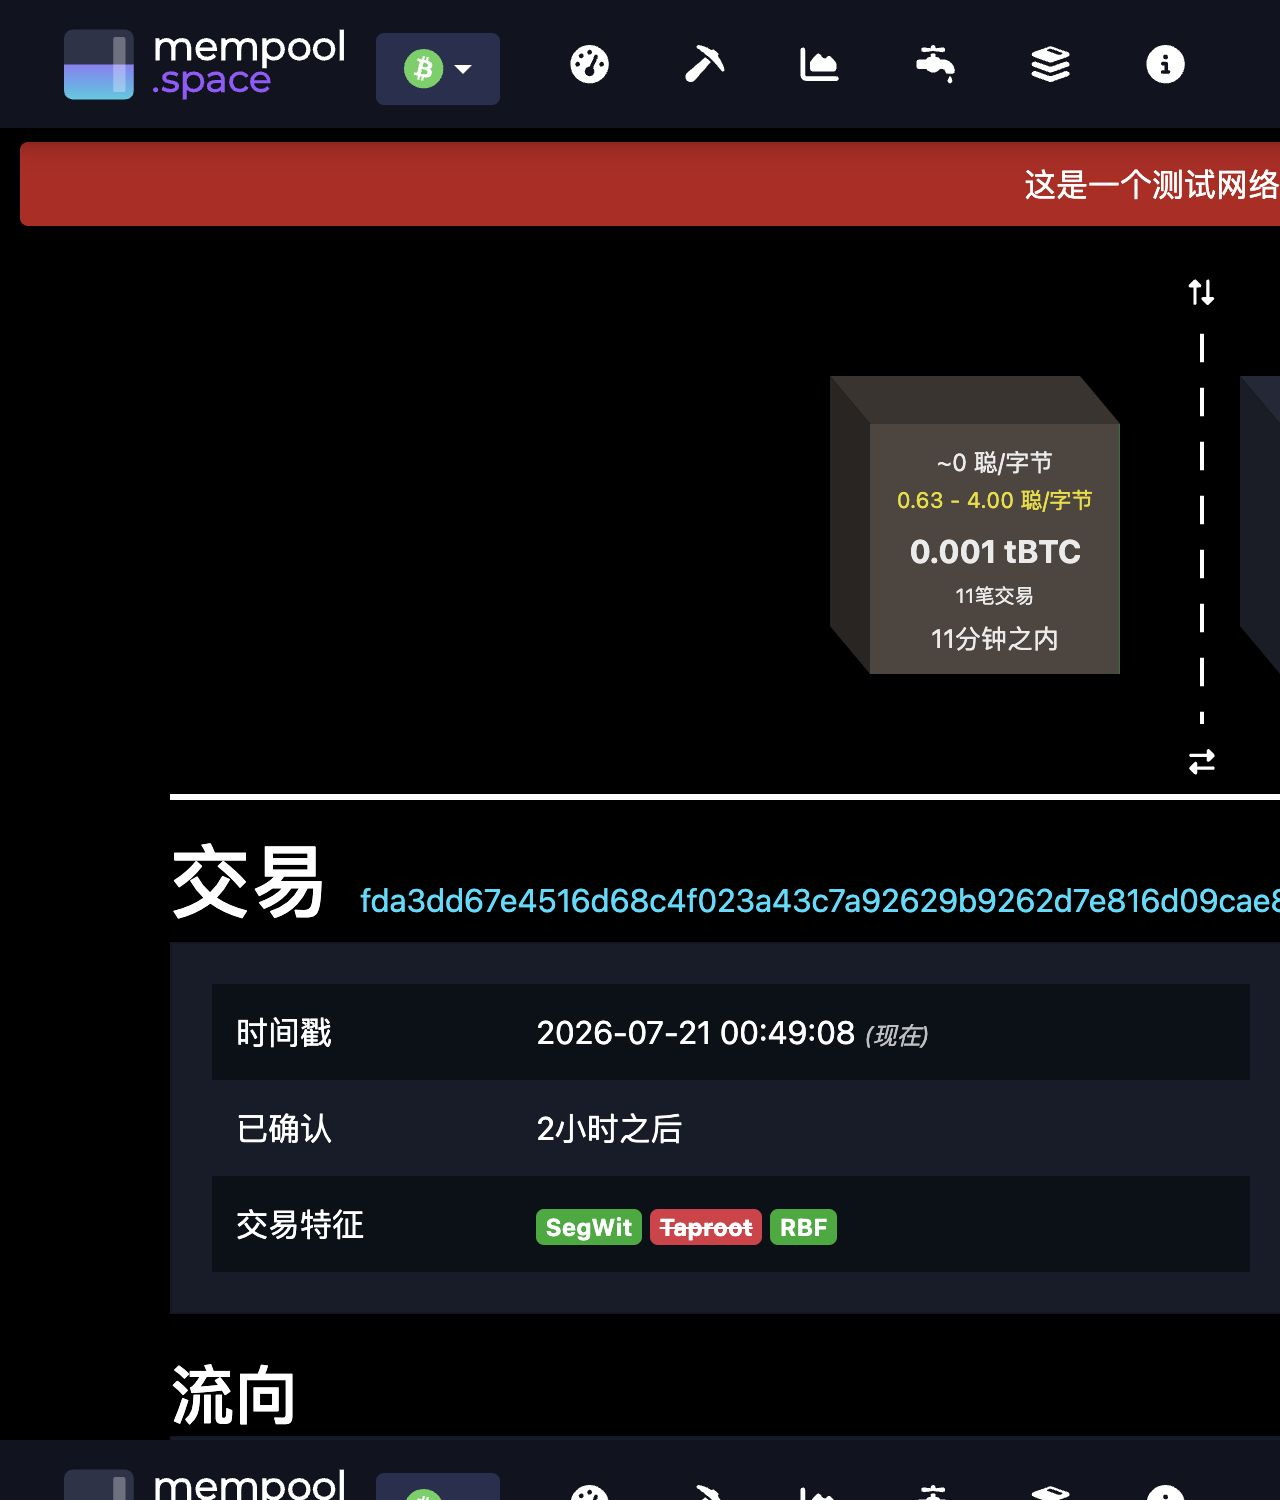
\includegraphics[width=\linewidth,height=0.20\textheight,keepaspectratio]{assets/testnet4_experiment_tx_confirmed.png}
  \caption{实验交易进入高度 144927 并确认}
\end{subfigure}\hfill
\begin{subfigure}[t]{0.48\textwidth}
  \centering
  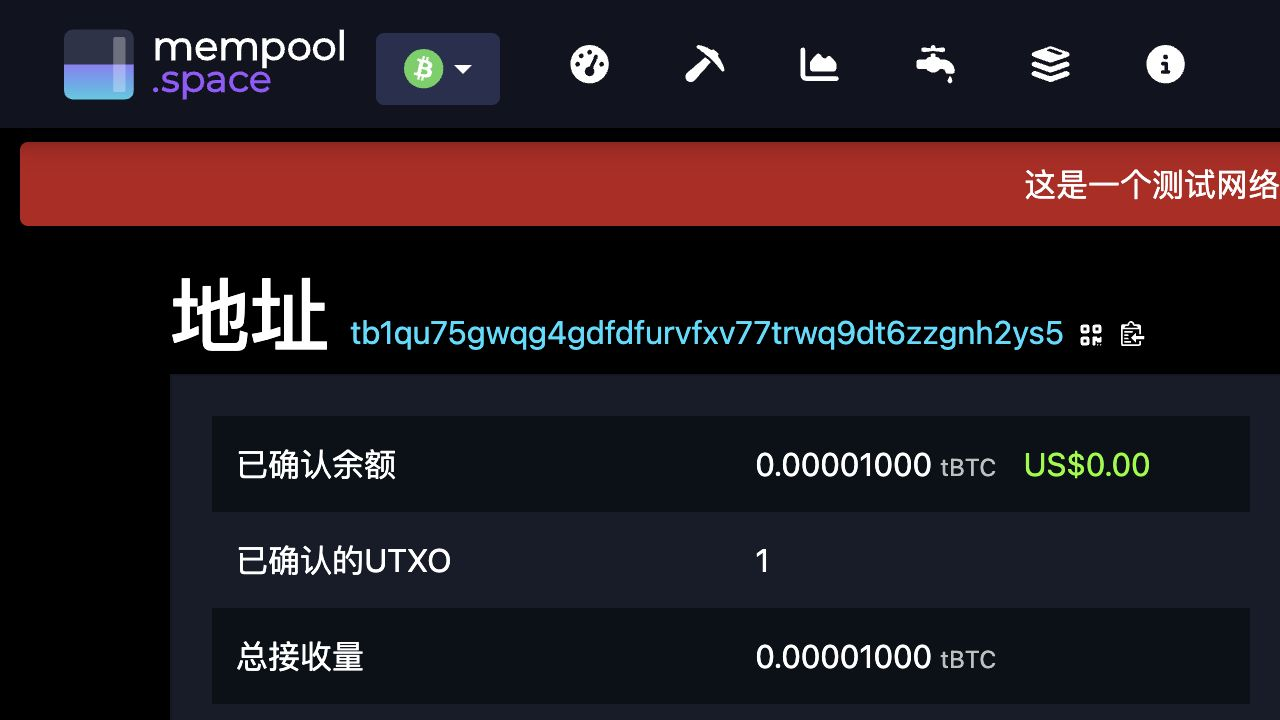
\includegraphics[width=\linewidth,height=0.20\textheight,keepaspectratio]{assets/testnet4_receiver_confirmed.png}
  \caption{Receiver 最终余额与已确认 UTXO}
\end{subfigure}
\caption{从 Faucet 入账、实验交易广播到最终确认的完整公开链上过程}
\label{fig:tx-process}
\end{figure}

\clearpage
完整复现命令为：
\begin{lstlisting}[language=bash]
.venv/bin/btc-lab funding-status
.venv/bin/btc-lab build --payment-sats 1000 --fee-rate 2
.venv/bin/btc-lab broadcast
.venv/bin/btc-lab fetch-confirmation
.venv/bin/btc-lab verify
\end{lstlisting}
若交易持续未确认，可在确认其仍位于 mempool 后运行下列命令，使用同一输入构造 opt-in RBF 替代交易：
\begin{lstlisting}[language=bash]
.venv/bin/btc-lab build --fee-rate 10 --replace-draft
\end{lstlisting}

\section{测试、限制与结论}

\subsection{分层测试与验收证据}

17 个自动化测试与真实链上集成验证分工如下。单元测试负责在小输入上精确定位边界错误；真实交易与完整区块则证明同一实现可以处理生产规模的组合结构。

\begin{table}[H]
\centering
\caption{测试层次与失败时可定位的问题}
\label{tab:task1-tests}
\begin{tabular}{p{0.25\textwidth}p{0.38\textwidth}p{0.27\textwidth}}
\toprule
测试对象 & 关键用例 & 验收条件 \\
\midrule
CompactSize/整数 & 252/253、65,535/65,536，non-canonical、truncated & 值和消费长度正确；非法输入明确拒绝 \\
交易解析 & legacy、SegWit、空 scriptSig、trailing bytes & TXID/WTXID、size、weight、最终 offset 正确 \\
Script 反汇编 & 直接 push、PUSHDATA1/2/4、未知 opcode、截断 push & 数据边界不越界，未知 opcode 不丢失 \\
签名验证 & 合成 P2WPKH 与真实 witness & BIP143 digest、DER、low-S、ECDSA 全部通过 \\
区块解析 & coinbase、奇数 Merkle 层、witness commitment & block hash、Merkle、PoW、承诺全部通过 \\
逐字节覆盖 & 223-byte 交易与 88,989-byte 区块 & 无缺口、无重叠、每条 bits 长度为 8 \\
\bottomrule
\end{tabular}
\end{table}

真实验收还进行了跨来源对照：本地计算的 TXID、WTXID、block hash、height、金额、手续费、weight/vsize 与 Testnet4 公共数据一致；交易确实出现在高度 144927 的原始区块第 8 笔；\texttt{btc-lab verify} 可执行的检查均为 true。因而验收不依赖单个截图或单个 API 字段。

\subsection{范围与限制}

本工具的目标是课程实验所需的序列化、常见脚本识别和本次 P2WPKH 验证，不是 Bitcoin Core 的替代实现。它没有覆盖所有历史 sighash 特例、软分叉激活状态、Script 数值规则、资源限制和 Taproot script-path 共识语义；完整区块中其他输入只做结构解析，不据此声称重新执行了整个 UTXO 状态转换。Esplora API 仍承担 UTXO 发现、广播与原始数据传输，但所有密码学与字节级结论都由下载后的 raw bytes 本地复算。Testnet4 资产没有经济价值，实验密钥也不得迁移到主网使用。

\subsection{结论}

交易/区块序列化不是“读取 explorer JSON”，而是以原始字节为唯一输入，显式处理 CompactSize、端序、witness 与哈希展示约定，并用可独立复算的 BIP143 摘要、ECDSA、TXID/WTXID、Merkle root、witness commitment 和 PoW 建立闭环。本实验已从 faucet UTXO、交易构造、广播、确认到完整确认区块逐字节解析全部贯通；223-byte 交易与 88,989-byte 区块均达到每字节一个 8-bit 归属记录。完整 JSON、CSV 和 raw hex 保存在 \texttt{output/data} 与 \texttt{data/raw}，私钥始终只存在于权限 0600 且被忽略的秘密文件中。

\begin{thebibliography}{9}
\bibitem{txref} Bitcoin Developer Reference, \emph{Transactions}. \url{https://developer.bitcoin.org/reference/transactions.html}
\bibitem{blockref} Bitcoin Developer Reference, \emph{Block Chain}. \url{https://developer.bitcoin.org/reference/block_chain.html}
\bibitem{bip141} BIP 141, \emph{Segregated Witness}. \url{https://github.com/bitcoin/bips/blob/master/bip-0141.mediawiki}
\bibitem{bip143} BIP 143, \emph{Transaction Signature Verification for Version 0 Witness Program}. \url{https://github.com/bitcoin/bips/blob/master/bip-0143.mediawiki}
\bibitem{bip34} BIP 34, \emph{Block v2, Height in Coinbase}. \url{https://github.com/bitcoin/bips/blob/master/bip-0034.mediawiki}
\bibitem{bip94} BIP 94, \emph{Testnet 4}. \url{https://github.com/bitcoin/bips/blob/master/bip-0094.mediawiki}
\bibitem{core28} Bitcoin Core 28.0 Release Notes, Testnet4 support. \url{https://bitcoincore.org/en/releases/28.0/}
\end{thebibliography}

\end{document}
